%% LyX 2.4.0~beta5 created this file.  For more info, see https://www.lyx.org/.
%% Do not edit unless you really know what you are doing.
\documentclass[english,footrule]{foils}
\usepackage[T1]{fontenc}
\usepackage[latin9]{inputenc}
\pagestyle{foilheadings}
\setcounter{secnumdepth}{1}
\setcounter{tocdepth}{1}
\usepackage{xcolor}
\usepackage{pdfpages}
\usepackage{amsmath}
\usepackage{amsthm}
\usepackage{amssymb}
\usepackage{graphicx}

\makeatletter

%%%%%%%%%%%%%%%%%%%%%%%%%%%%%% LyX specific LaTeX commands.
%% A simple dot to overcome graphicx limitations
\newcommand{\lyxdot}{.}


%%%%%%%%%%%%%%%%%%%%%%%%%%%%%% Textclass specific LaTeX commands.
\theoremstyle{definition}
\newtheorem{defn}{\protect\definitionname}
\theoremstyle{remark}
\newtheorem{rem}{\protect\remarkname}
\newenvironment{lyxcode}
	{\par\begin{list}{}{
		\setlength{\rightmargin}{\leftmargin}
		\setlength{\listparindent}{0pt}% needed for AMS classes
		\raggedright
		\setlength{\itemsep}{0pt}
		\setlength{\parsep}{0pt}
		\normalfont\ttfamily}%
	 \item[]}
	{\end{list}}
\theoremstyle{remark}
\newtheorem*{rem*}{\protect\remarkname}
\theoremstyle{plain}
\newtheorem{thm}{\protect\theoremname}

%%%%%%%%%%%%%%%%%%%%%%%%%%%%%% User specified LaTeX commands.
\usepackage{xcolor}
\renewcommand{\labelitemi}{$\textcolor{blue}{\bullet}$}
\renewcommand{\labelitemii}{$\textcolor{teal}{\Rightarrow}$}
\renewcommand{\labelitemiii}{$\textcolor{red}{\rightarrow}$}
\renewcommand{\labelitemiv}{$\textcolor{brown}{\circ}$}
% for French theorems, etc. since I'm using English to fix bullet pb.
\providecommand{\examplename}{Example}
\providecommand{\definitionname}{Definition}
\providecommand{\theoremnname}{Theorem}
\providecommand{\remarkname}{Remark}
\providecommand{\exercisename}{Exercise}
% DT book stuff
\newcommand{\argmin}{\operatornamewithlimits{argmin}} % for a "clean" argmin 
\newcommand{\T}{\mathrm{T}}  % transpose
\newcommand{\PP}{\mathrm{P}}  % probability
\newcommand{\dd}{\mathrm{d}} % integration dx
\newcommand{\ee}{\mathrm{e}} % exponential
\newcommand{\E}{\mathrm{E}} % expectation
%_%_%_%_%_%_%_%_
% for tikz drawings and cartoons
%_%_%_%_%_%_%_%_

\usepackage{tikz}

% for tikzit drawings
\usepackage{tikzit}
\input{flow.tikzstyles}


% for decision trees:
\tikzset{
	treenode/.style = {shape=rectangle, rounded corners,
		draw, align=center,
		top color=white, bottom color=blue!20},
	root/.style     = {treenode, font=\Large, bottom color=red!30},
	env0/.style     = {treenode, font=\large, bottom color=orange!30},
	env1/.style     = {treenode,  bottom color=green!30},
	env/.style      = {treenode, font=\ttfamily\normalsize},
    leaf/.style      = {treenode, font=\ttfamily\normalsize},
	dummy/.style    = {circle,draw}
}
\usetikzlibrary{positioning}



\usepackage{tcolorbox}

%_%_%_%_%_%_%_%_%_%_
% for algorithms and listings
%_%_%_%_%_%_%_%_%_%_

%\usepackage{algorithm_MA,algpseudocode}
%\usepackage{algorithmic}
\usepackage{algpseudocode}

%\floatstyle{ruled}
%\newfloat{algorithm}{tbp}
%\providecommand{\algorithmname}{Algorithm}
%\floatname{algorithm}{\protect\algorithmname}
%

% try and fix \Comment problem due to excessive defs in Chap. DA
\algrenewcommand{\algorithmiccomment}[1]{%
	\hfill$\triangleright$\ \textcolor{darkgray}{#1}}

\makeatother

\usepackage{babel}
\providecommand{\definitionname}{Definition}
\providecommand{\remarkname}{Remark}
\providecommand{\theoremname}{Theorem}

\begin{document}

\MyLogo{SciML - ML techniques}
\title{SciML - Machine learning\\
\rule[0.5ex]{1\columnwidth}{3pt}}
\author{Mark Asch - IMU/VLP/CSU }
\date{2023}
\maketitle

\foilhead{Program}

Recall machine learning (ML) techniques for scientific applications
(see \textcolor{blue}{Basic Course} for details):
\begin{enumerate}
\item \textcolor{red}{General principles of ML.}
\begin{enumerate}
\item Under- and Over-fitting
\item Bias-Variance Tradeoff
\item Recall-Precision Tradeoff
\item Cross Validation
\end{enumerate}
\item Supervised learning:
\begin{enumerate}
\item Regression.
\item Classification.
\end{enumerate}
\item Unsupervised learning:
\begin{enumerate}
\item Clustering.
\item Trees.
\end{enumerate}
\item Surrogate models and dimensionality reduction.
\item The use of machine learning in scientific applications.
\item The challenges of applying machine learning to scientific applications.
\end{enumerate}

\foilhead{A simple example that brings out many points}
\begin{itemize}
\item Basic fact: most of ML is about \textcolor{magenta}{pattern recognition}---see
C. M. Bishop, PRML, Springer, 2006.
\begin{itemize}
\item we have a bunch of data, $\mathbf{x}$ and corresponding observations,
$\mathbf{y}$ 
\item we seek the relation (recognize the pattern), $f,$ that relates $\mathbf{x}$
to $\mathbf{y}$ 
\[
\mathbf{y}=f(\mathbf{x}),
\]
or,
\[
f\colon\mathbf{x}\longmapsto\mathbf{y}
\]
\item our goal: make \textcolor{red}{predictions} for new (unseen) data
(inputs)
\end{itemize}
\end{itemize}

\foilhead{Polynomial Curve Fitting}
\begin{itemize}
\item suppose that 
\[
y=\sin(2\pi x)+\mathrm{noise}
\]
\item given: a \textcolor{magenta}{training} set of $N$ observations of
$x$, 
\[
\mathbf{x}=\left[\begin{array}{c}
x_{1}\\
x_{2}\\
\vdots\\
x_{N}
\end{array}\right]
\]
and the corresponding (noisy) \textcolor{magenta}{observations},
\[
\mathbf{y}=\left[\begin{array}{c}
y_{1}\\
y_{2}\\
\vdots\\
y_{N}
\end{array}\right]
\]
\end{itemize}
\begin{center}
\includegraphics[width=0.8\textwidth]{\string"/Users/markasch/Documents/Refs/Statistics and Data Science/Bishop-PRML/prmlfigs-eps/Figure1.2\string".pdf}
\par\end{center}
\begin{itemize}
\item data generation from
\[
y_{i}=\sin(2\pi x_{i})+\epsilon,
\]
 where the noise term,
\[
\epsilon\thicksim\mathcal{N}(0,\sigma)
\]
is due to intrinsic/natural variability and other uncertainties from
the data collection methods.
\item \textbf{\textcolor{magenta}{Objective:}}\textcolor{magenta}{{} }from
the training set, learn/discover an approximation of the relation
$f$ that will enable us to make predictions based on
\begin{itemize}
\item probability theory
\item (polynomial) curve fitting
\end{itemize}
\item PCF: suppose that the data can be represented by the\textcolor{magenta}{{}
polynomial/''linear model''}
\[
y(x,\mathbf{w})=w_{0}+w_{1}x+w_{2}x^{2}+\cdots+w_{M}x^{M}=\sum_{k=0}^{M}w_{k}x^{k}
\]
 with \textcolor{magenta}{weight} vector (coefficients) $\mathbf{w}.$
\begin{itemize}
\item compute the coefficents by minimizing an \textcolor{magenta}{error/loss
function}---this is (often) a least-squares approach, where the loss
function is defined as
\[
\mathcal{L}(\mathbf{w})=\frac{1}{2}\sum_{i=1}^{N}\left[\hat{y}(x_{i},\mathbf{w})-y_{i}\right],
\]
where $\hat{y}_{i}$ is the approximation obtained from our polynomial
model.
\end{itemize}
\end{itemize}
\begin{center}
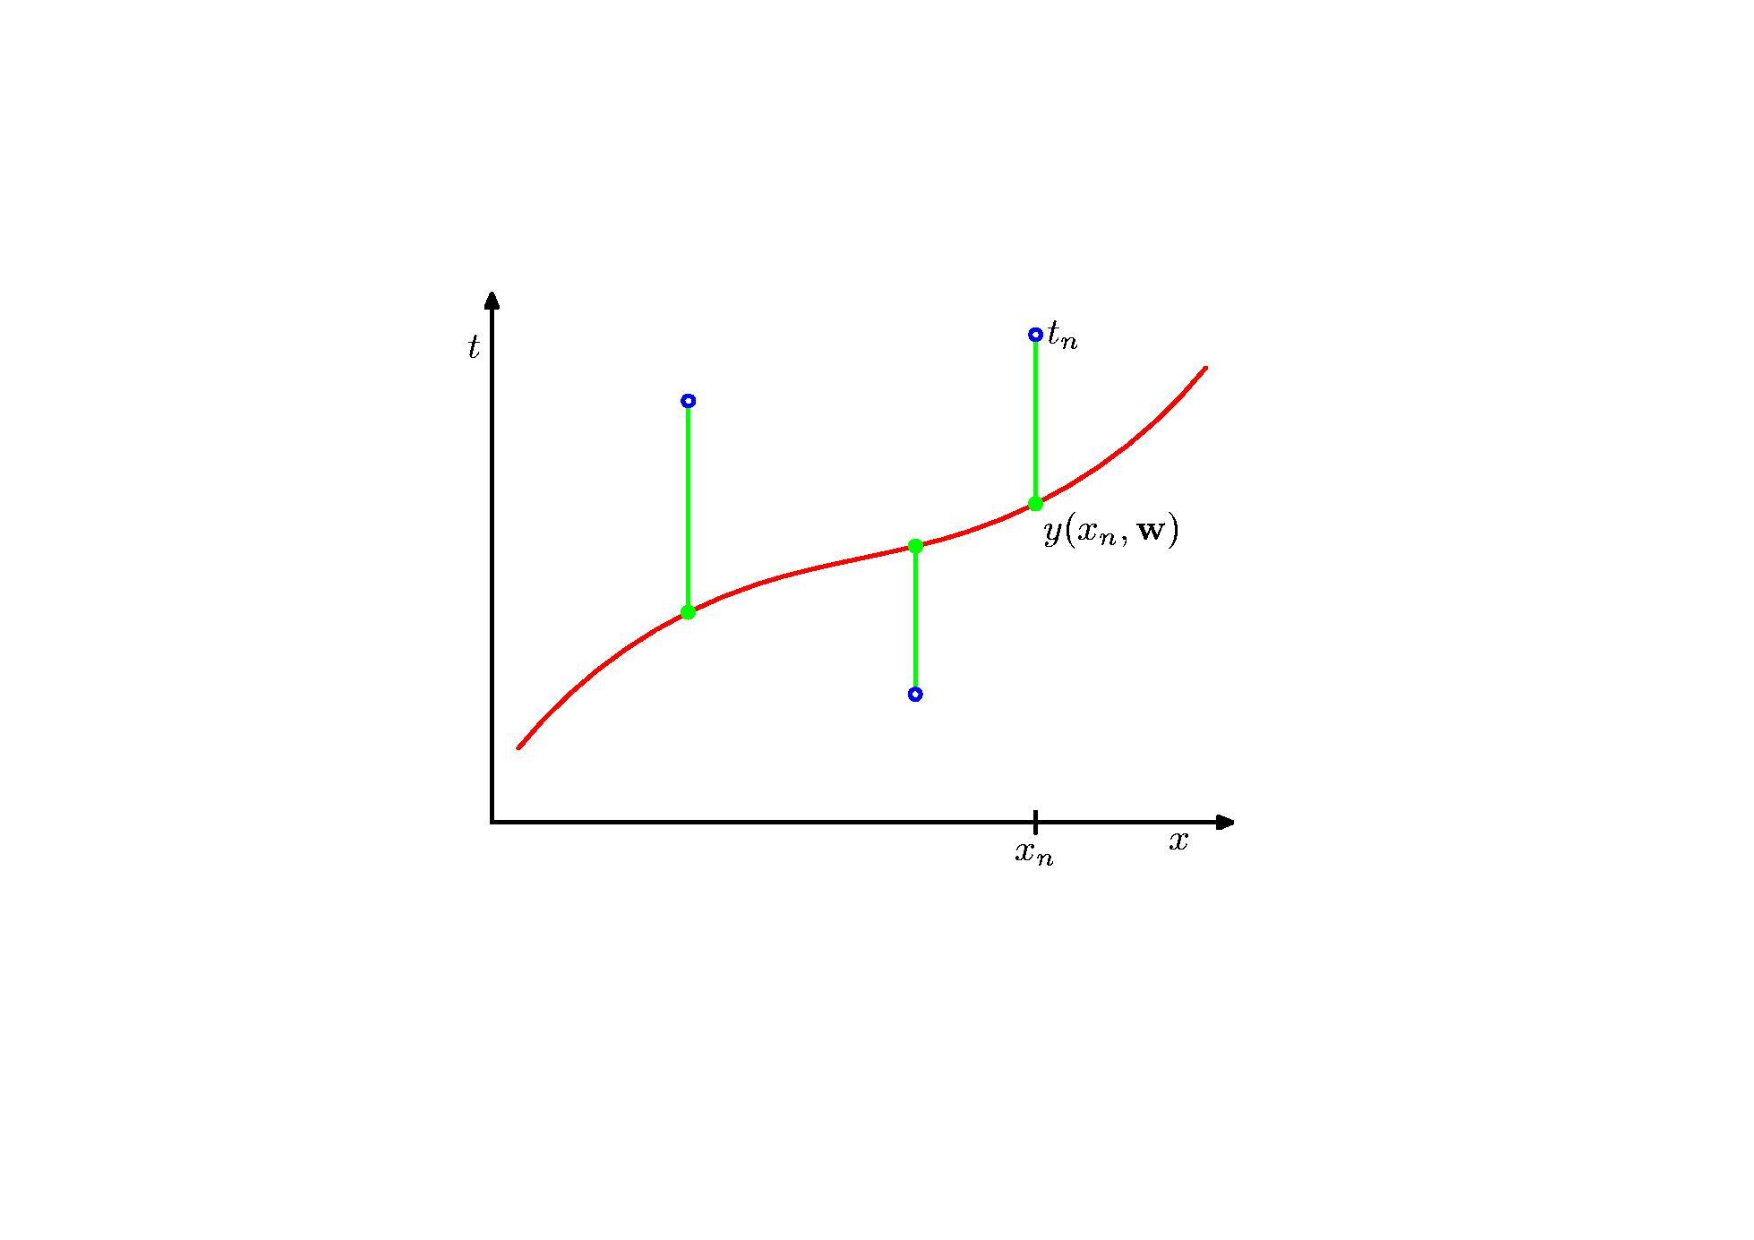
\includegraphics[width=0.8\textwidth]{graphics/prml-slides-1}
\par\end{center}
\begin{itemize}
\item in the case of a quadratic loss function, the gradient is linear and
the solution to the optimization problem exists and can be found in
closed form using the normal form, or psuedo-inverse,
\[
\mathbf{w}_{*}=\left(X^{\mathrm{T}}X\right)^{-1}X^{\mathrm{T}}\mathbf{y},
\]
 where $X$ is the (rectangular) coefficient matrix of dimension $(N\times M)$
with $N>M$ and $\mathbf{y}$ is the data/observation vector.
\item the choice of $M$ is a\textcolor{magenta}{{} model selection} problem
\begin{itemize}
\item we compute the solution for $4$ values: $M=0,1,3,9$---see below
\item Model $M=0$ produces \textcolor{magenta}{underfitting}---it is too
simple and does not find the trend 
\item Model $M=P$ produces \textcolor{magenta}{overfitting}---it fits
the data points perfectly, but is ``brittle'' and does not generalize 
\end{itemize}
\item \textbf{Conclusion:} we must seek a \textcolor{magenta}{compromise}
between the two.
\end{itemize}
\includepdf[pages=-,scale=1.2]{02a_prml-slides-2}

\foilhead{Bias-Variance Compromise}
\begin{itemize}
\item We saw the dangers of \textcolor{red}{overfitting} in the very simple
polynomial fitting example. 
\item To treat this, we need to make a \textcolor{magenta}{compromise} between
bias and variance, i.e. forgo some precision in order to attain better
\textcolor{magenta}{predictive performance.} 
\begin{itemize}
\item this is a fundamental point underlying \textbf{\textcolor{red}{ALL}}
machine learning methods
\end{itemize}
\end{itemize}
\begin{center}
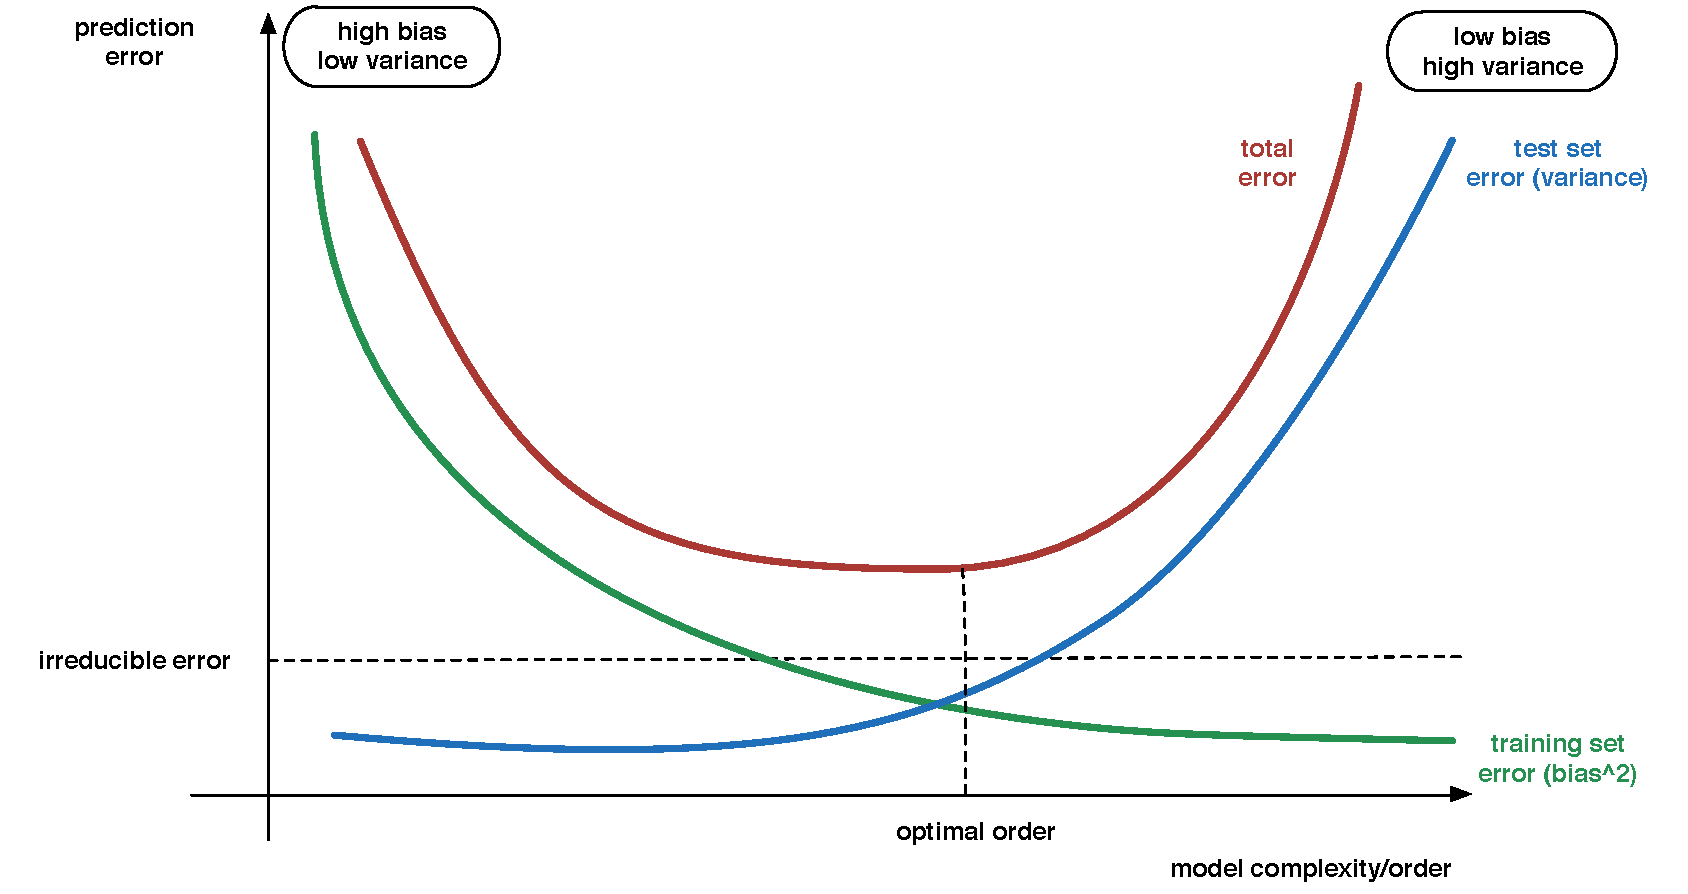
\includegraphics[width=1\textwidth]{graphics/bias-variance-eps-converted-to}
\par\end{center}

\foilhead{Recall: Mean-Squared Error}
\begin{itemize}
\item Since we are estimating an unknown parameter, or more often, unknown
function, we need to evaluate 
\begin{itemize}
\item how good our estimation is?
\item the quality of the estimation?
\end{itemize}
\item This is traditionally done by using a discrete $L_{2}$ norm, though
other norms are possible and are used in specific circumstances---see
below.
\item Before defining the MSE, we need to recall the definitions of
\begin{itemize}
\item \textcolor{magenta}{expectation} (or expected value): $\mathrm{E}[X]=\sum_{i}x_{i}f(x_{i}),$
where $f$ is the (discrete) probability function.
\item \textcolor{magenta}{bias}: $\mathrm{Bias}(T,\theta)=\mathrm{Bias}(T)=\mathrm{E}[T]-\theta,$
where $T$ is a statistic used to estimate a parameter, and $\theta$
is the parameter to be estimated
\item \textcolor{magenta}{variance}: $\mathrm{Var}\left[X\right]=\mathrm{E}\left[(X-\mu)^{2}\right]=\mathrm{E}\left[X^{2}\right]-\mu^{2},$
where $\mu$ is the mean of $X.$ 
\end{itemize}
\end{itemize}
\begin{defn}
[Mean Squared Error]The mean squared error measures the \textcolor{magenta}{average
of the squares of the errors}---that is, the average squared difference
between the estimated values and the actual value. MSE is a risk function,
corresponding to the expected value of the squared error loss.
\[
\mathrm{MSE}=\frac{1}{n}\sum_{i=1}^{n}\left(y_{i}-\hat{y}_{i}\right)^{2}=\frac{1}{n}\sum_{i=1}^{n}\left(e_{i}\right)^{2},
\]
or for an estimator
\[
\mathrm{MSE}(\hat{\theta})=\mathrm{E}_{\theta}\left[\left(\hat{\theta}-\theta\right)^{2}\right].
\]

The MSE is the second moment (about the origin) of the error, and
thus incorporates both the \textcolor{magenta}{variance} of the estimator
(how widely spread the estimates are from one data sample to another)
and its \textcolor{magenta}{bias} (how far off the average estimated
value is from the true value).

The MSE either assesses the quality of a\textcolor{magenta}{{} predictor}
(i.e., a function mapping arbitrary inputs to a sample of values of
some random variable), or of an \textcolor{magenta}{estimator} (i.e.,
a mathematical function mapping a sample of data to an estimate of
a parameter of the population from which the data is sampled). The
definition of an MSE differs according to whether one is describing
a predictor or an estimator.
\end{defn}
\begin{rem}
The mean squared error has the disadvantage of heavily weighting \textcolor{magenta}{outliers}.
This is a result of the squaring of each term, which effectively weights
large errors more heavily than small ones. This property, undesirable
in many applications, has led to the use alternatives such as the
\textcolor{magenta}{mean absolute error}, which is a discrete $L_{1}$
norm, or those based on the median.
\end{rem}
\begin{defn}
[Mean Absolute Error]The mean absolute error is the average of the
sum of absolute errors,
\[
\mathrm{MAE}=\frac{1}{n}\sum_{i=1}^{n}\left|y_{i}-\hat{y}_{i}\right|=\frac{1}{n}\sum_{i=1}^{n}\left|e_{i}\right|,
\]
or for an estimator
\end{defn}
\begin{itemize}
\item A python snippet:
\end{itemize}
\begin{lyxcode}
\textcolor{teal}{from~sklearn.metrics~import~mean\_absolute\_error~}

\textcolor{teal}{import~numpy~as~np}

\textcolor{teal}{\#~Generate~some~sample~data}

\textcolor{teal}{y\_true~=~np.array({[}1,~2,~3,~4,~5{]})}

\textcolor{teal}{y\_pred~=~np.array({[}1.5,~2.5,~2.8,~4.2,~4.9{]})}

\textcolor{teal}{\#~Calculate~the~MAE}

\textcolor{teal}{mae~=~mean\_absolute\_error(y\_true,~y\_pred)}

\textcolor{teal}{print(\textquotedbl Mean~Absolute~Error\textquotedbl ,~mae)}
\end{lyxcode}
\begin{rem*}
The MAE has two important properties. It is robust to outliers, and
it has the same units as the response variable.
\end{rem*}

\foilhead{Bias-Variance Decomposition of MSE}
\begin{thm}
The bias-variance decomposition of the MSE is given by
\begin{align*}
\mathrm{MSE} & \doteq\mathrm{E}\left[\left(y-\hat{f}\right)^{2}\right]\\
 & =\mathrm{Bias}\left[\hat{f}\right]^{2}+\mathrm{Var}\left[\hat{f}\right]+\sigma^{2},
\end{align*}
where $y=f(x)+\epsilon,$ $\epsilon\sim\mathcal{N}(0,\sigma^{2})$
and $\hat{f}(x)$ is an approximation/model of the true (unknown)
function $f(x)$. 
\end{thm}
\begin{proof}
First expand the definition of MSE,
\begin{align*}
\mathrm{MSE} & \doteq\mathrm{E}\left[\left(y-\hat{f}\right)^{2}\right]\\
 & =\mathrm{E}\left[y^{2}-2y\hat{f}+\hat{f}^{2}\right]\\
 & =\mathrm{E}\left[y^{2}\right]-2\mathrm{E}\left[y\hat{f}\right]+\mathrm{E}\left[\hat{f}^{2}\right].
\end{align*}
Now look at each of the three terms.
\[
\mathrm{E}\left[\hat{f}^{2}\right]=\mathrm{Var}\left[\hat{f}\right]+\mathrm{E}\left[\hat{f}\right]^{2}
\]
from variance decomposition.
\begin{align*}
\mathrm{E}\left[y^{2}\right] & =\mathrm{E}\left[\left(f+\epsilon\right)^{2}\right]\\
 & =\mathrm{E}\left[f^{2}\right]+2\mathrm{E}\left[f\epsilon\right]+\mathrm{E}\left[\epsilon^{2}\right]\\
 & =f^{2}+2f\cdot0+\sigma^{2}
\end{align*}
from definition of the noise distribution $\epsilon.$
\begin{align*}
\mathrm{E}\left[y\hat{f}\right] & =\mathrm{E}\left[\left(f+\epsilon\right)\hat{f}\right]\\
 & =\mathrm{E}\left[f\hat{f}\right]+\mathrm{E}\left[\epsilon\right]\mathrm{E}\left[\hat{f}\right]\\
 & =f\mathrm{E}\left[\hat{f}\right].
\end{align*}
Putting it all together, we find
\begin{align*}
\mathrm{MSE} & =\left(f^{2}+\sigma^{2}\right)-2f\mathrm{E}\left[\hat{f}\right]+\left(\mathrm{Var}\left[\hat{f}\right]+\mathrm{E}\left[\hat{f}\right]^{2}\right)\\
 & =\left(f-\mathrm{E}\left[\hat{f}\right]\right)^{2}+\sigma^{2}+\mathrm{Var}\left[\hat{f}\right]\\
 & =\mathrm{Bias}\left[\hat{f}\right]^{2}+\mathrm{Var}\left[\hat{f}\right]+\sigma^{2}.
\end{align*}
\end{proof}

\foilhead{Bias-Variance Compromise II}
\begin{itemize}
\item Questions:
\begin{itemize}
\item What is bias? (see also \textcolor{magenta}{Ethics} lecture) 
\begin{itemize}
\item \textcolor{magenta}{Low Bias}: Predicted data points are close to
the target. The model has fewer assumptions about the form of the
target function. 
\item \textcolor{magenta}{High-Bias}: Predicted data points are far from
the target. The model has more assumptions about the form of the target
function.
\end{itemize}
\item What is variance?
\begin{itemize}
\item \textcolor{magenta}{Low Variance}: Data points are close to each other,
and as a result are close to the function. The model suggests small
changes to the estimate of the target function with changes in the
training dataset. 
\item \textcolor{magenta}{High Variance}: Data points are spread out and
as a result are far from the function. The model suggests large changes
to the estimate of the target function with changes in the training
dataset.
\end{itemize}
\end{itemize}
\end{itemize}
\begin{center}
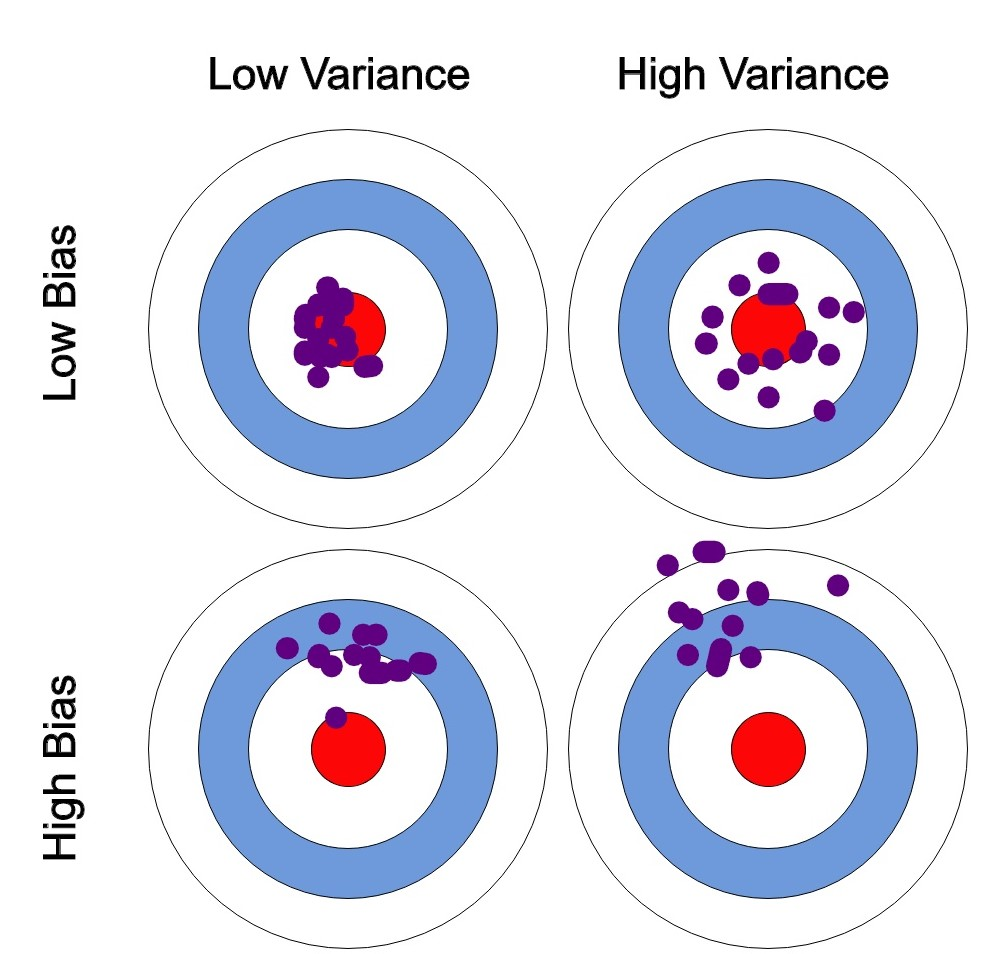
\includegraphics[width=0.9\textwidth]{graphics/bias_variance}
\par\end{center}

\foilhead{Bias-Variance Compromise III}
\begin{itemize}
\item We can now return to the question of the \textcolor{magenta}{tradeoff}
between bias and variance.
\item Looking at the bias-variance decomposition of the MSE,
\[
\mathrm{MSE}=\mathrm{Bias}\left[\hat{f}\right]^{2}+\mathrm{Var}\left[\hat{f}\right]+\sigma^{2},
\]
 we observe that we need to simultaneously minimize both bias and
variance. This is the \textcolor{magenta}{reducible} part of the error,
whereas $\sigma^{2}$ is the intrinsic, \textcolor{magenta}{irreducible}
part and cannot be reduced by the ML model.
\item Theoretical result (see also the ``compromise curve'' above):
\begin{itemize}
\item Decreasing the bias will mechanically increase the variance. 
\begin{itemize}
\item Low bias $\Longrightarrow$ high variance.
\end{itemize}
\item Decreasing the variance will mechanically increase the bias. 
\begin{itemize}
\item Low variance $\Longrightarrow$ high bias.
\end{itemize}
\end{itemize}
\item \textbf{\textcolor{red}{Conclusion: }}
\begin{itemize}
\item To build a good model, we need to find a good balance/compromise/tradeoff
between bias and variance that minimizes the total/generalization
error. 
\item An optimal balance of bias and variance should neither overfit nor
underfit the model. This is achieved by hyperparameter tuning on the
basis of systematic grid-search (trial and error, or experience, for
the ranges) and cross-validation. See below, and examples.
\end{itemize}
\end{itemize}

\foilhead{Over- and Underfitting}
\begin{itemize}
\item ML Algorithm properties:
\begin{itemize}
\item Examples of\textcolor{magenta}{{} low-bias} machine learning algorithms:
Decision Trees, k-Nearest Neighbors and Support Vector Machines. 
\item Examples of \textcolor{magenta}{high-bias} machine learning algorithms:
Linear Regression, Linear Discriminant Analysis and Logistic Regression.
\item Examples of \textcolor{magenta}{low-variance} machine learning algorithms:
Linear Regression, Linear Discriminant Analysis and Logistic Regression. 
\item Examples of \textcolor{magenta}{high-variance} machine learning algorithms:
Decision Trees, k-Nearest Neighbors and Support Vector Machines.
\end{itemize}
\item Dealing with the overfitting problem:
\begin{itemize}
\item always be prepared to ``sacrifice'' some bias, to get a lower variance,
since it is the variance that is the most ``dangerous'' in terms of
\textcolor{magenta}{predictive power/performance.}
\item in general, prefer lower-order ML methods---so-called \textcolor{magenta}{linear
methods}
\item increase the number of \textcolor{magenta}{data points}---this is
not always feasible in reality
\item use a \textcolor{magenta}{Bayesian} approach---probably the best,
but more complex to implement
\item \textcolor{magenta}{regularize} the problem---penalize terms of large
magnitude, but requires extrensive tuning of the regularization parameters
that usually relies on \textcolor{magenta}{cross-validation} techniques.
\end{itemize}
\end{itemize}

\foilhead{BV Tradeoff: Double Descent phenomenon}
\begin{itemize}
\item Test error can present a ``double descent'' phenomenon in a range
of ML models.
\item As the number of model parameters grows relative to the number of
data points, test error drops in the highly \textcolor{magenta}{overparameterized}
(data undersampled) regime
\end{itemize}
\begin{center}
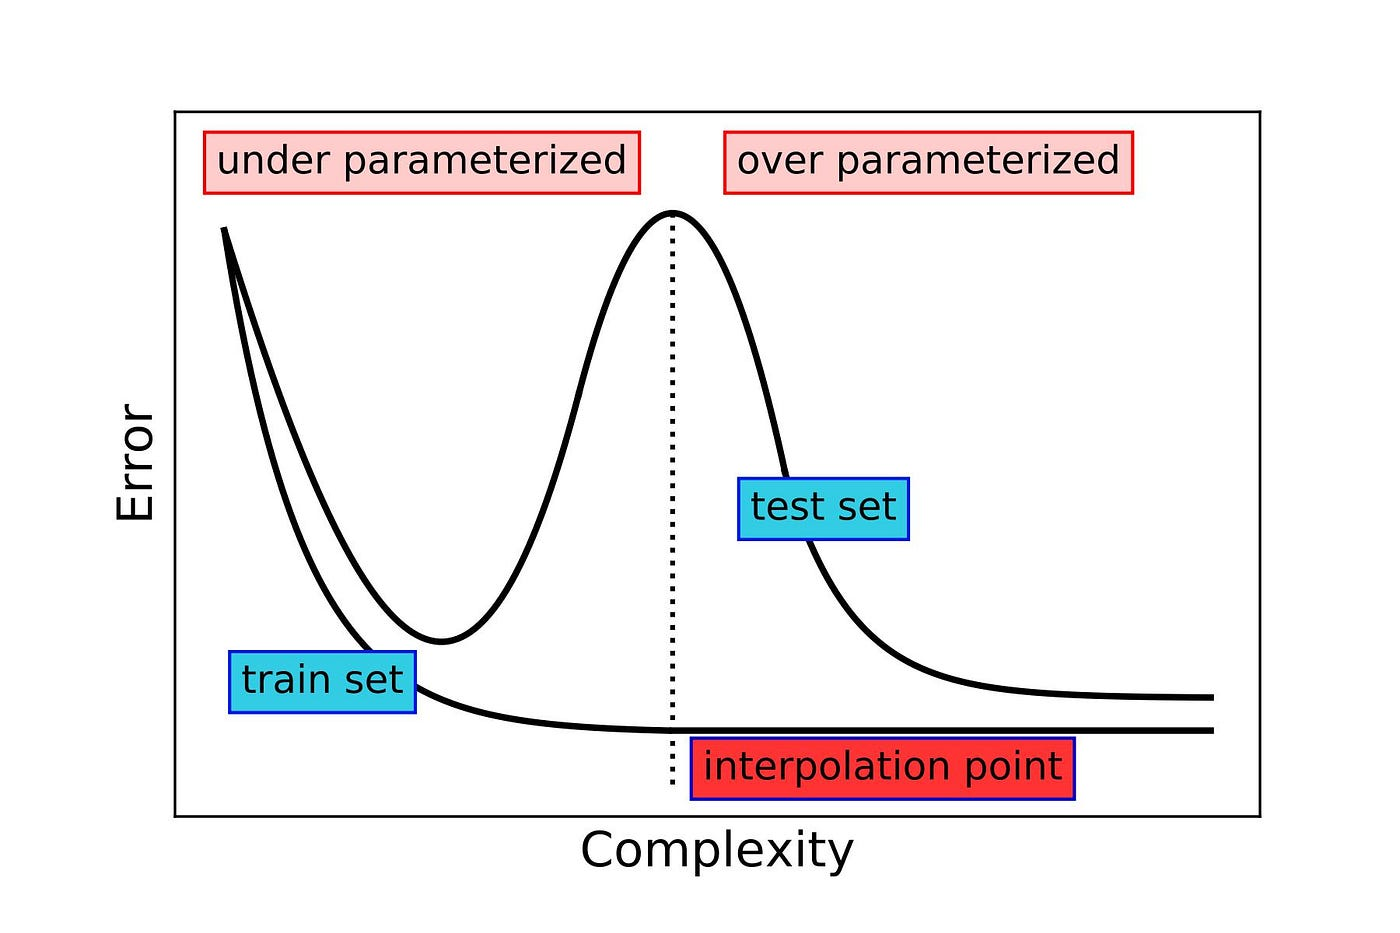
\includegraphics[width=0.9\textwidth]{graphics/double-descent_simple}
\par\end{center}
\begin{itemize}
\item Interpretation: {[}OpenAI{]}
\begin{itemize}
\item For models at the interpolation threshold, there is effectively only
one model that fits the train data, and forcing it to fit even slightly
noisy or misspecified labels will destroy its global structure.
\item There are no \textquotedblleft good models\textquotedblright{} which
both interpolate the train set and perform well on the test set. 
\item However, in the over-parameterized regime, there are many models that
fit the train set and there exist such good models. 
\item Moreover, the implicit bias of stochastic gradient descent (SGD) leads
it to such good models, for reasons we do not yet understand...
\end{itemize}
\end{itemize}

\foilhead{Precision-Recall Compromise}
\begin{itemize}
\item What happens with \textcolor{magenta}{binary classification} problems?
\begin{itemize}
\item the famous ``truth/confusion table'':
\begin{itemize}
\item True positives (TP): positive COVID test, correctly diagnosed.
\item False positives (FP): positive COVID test, falsely diagnosed.
\item True negatives (TN): negative COVID test, correctly diagnosed.
\item False negatives (FN): negative COVID test, falsely diagnosed.
\end{itemize}
\end{itemize}
\end{itemize}
\begin{center}
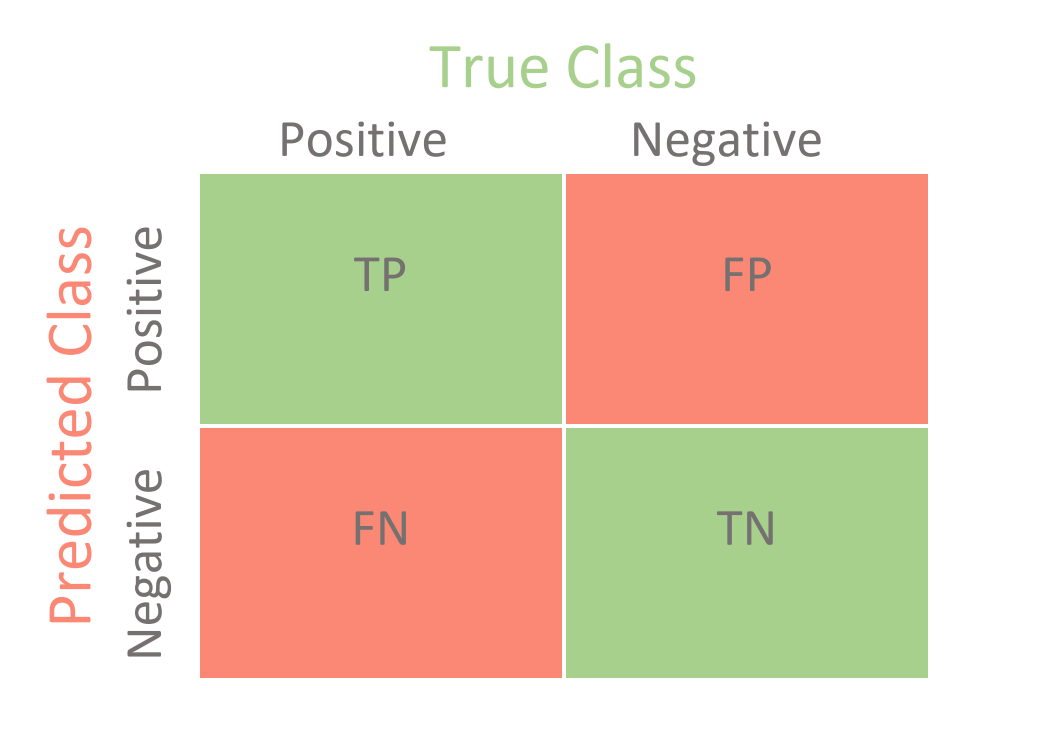
\includegraphics[width=0.6\textwidth]{graphics/confusion}
\par\end{center}
\begin{defn}
A \emph{confusion table/matrix }, $C$, for a classification with
$n$ classes is an $(n\times n)$ matrix with entries 
\begin{align*}
C_{ij} & =\mathrm{\,the\,number\,of\,observations\,in\,class}\,i\,\\
 & \,\,\,\,\,\,\,\,\,\,\mathrm{that\,are\,predicted\,in\,class}\,j.
\end{align*}
Then,
\end{defn}
\begin{itemize}
\item $C_{ii},$ $i=1,\ldots,n,$ are the \textcolor{magenta}{good} classifications, 
\item $C_{ij}$ with $i\neq j$ are the \textcolor{magenta}{bad} classifications. 
\end{itemize}
%
\begin{itemize}
\item Now we can define precision and recall/sensitivity.
\begin{description}
\item [{Precision}] the number of true positives divided by the total number
of true positives and false positives: 
\[
{\displaystyle \mathrm{PPV}={\frac{\mathrm{TP}}{\mathrm{TP}+\mathrm{FP}}}=1-\mathrm{FDR}}
\]

\begin{description}
\item [{\textcolor{magenta}{Appropriate}}] when minimizing false positives
is the focus---FP is more serious, think of a false postive cancer
diagnosis, and the heavy, unecessary treatment that follows.
\end{description}
\item [{Recall}] the number of correct positive predictions made out of
all positive predictions that could have been made: 
\[
\mathrm{TPR}={\frac{\mathrm{TP}}{\mathrm{P}}}={\frac{\mathrm{TP}}{\mathrm{TP}+\mathrm{FN}}}=1-\mathrm{FNR}
\]
 
\begin{description}
\item [{\textcolor{magenta}{Appropriate}}] when minimizing false negatives
is the focus---FN is more serious, think of missing a positive COVID,
that then goes on to infect many people.
\end{description}
\item [{Specificity}] is the number of true negatives divided by the total
number of true negatives and false positives:
\[
{\displaystyle \mathrm{TNR}={\frac{\mathrm{TN}}{\mathrm{N}}}={\frac{\mathrm{TN}}{\mathrm{TN}+\mathrm{FP}}}=1-\mathrm{FPR}}
\]
\item [{F1-Score}] is the harmonic mean of precision and recall: 
\[
{\displaystyle \mathrm{F}_{1}=2\times{\frac{\mathrm{PPV}\times\mathrm{TPR}}{\mathrm{PPV}+\mathrm{TPR}}}={\frac{2\mathrm{TP}}{2\mathrm{TP}+\mathrm{FP}+\mathrm{FN}}}}
\]

\begin{description}
\item [{Alone,}] neither precision or recall tells the whole story. We
can have excellent precision with terrible recall, or alternately,
terrible precision with excellent recall. F-measure provides a way
to express both concerns with a single score.
\end{description}
\end{description}
\end{itemize}

\foilhead{Precision-Recall Compromise II}
\begin{center}
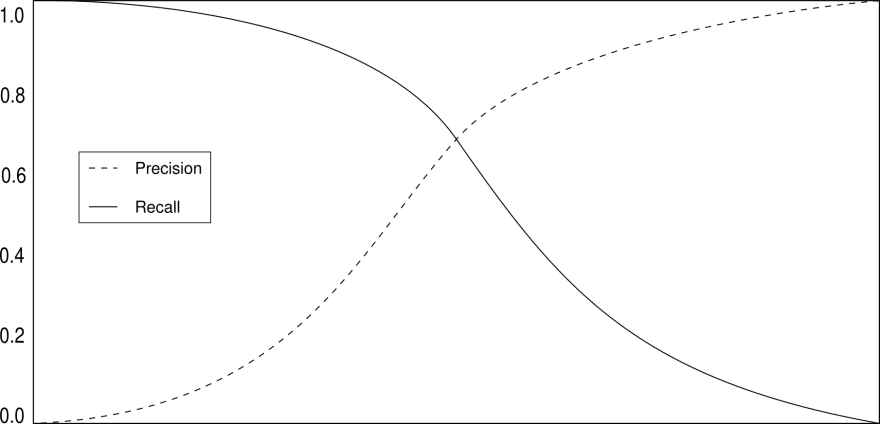
\includegraphics[width=0.6\textwidth]{graphics/prec_recall}
\par\end{center}
\begin{itemize}
\item The \textcolor{magenta}{compromise}: 
\begin{itemize}
\item When precision increases, recall decreases, and vice-versa. 
\item We cannot simultaneously increase both precision and recall.
\end{itemize}
\item To balance precision and recall, a number of \textcolor{magenta}{techniques}
can be used, such as 
\begin{itemize}
\item adjusting the decision threshold or 
\item using an ensemble of models. 
\end{itemize}
\item Another approach is to use a metric that combines both \textcolor{magenta}{precision
and recall}, 
\begin{itemize}
\item such as the F1 score, which is the harmonic mean of precision and
recall. 
\end{itemize}
\item Ultimately, the choice between precision and recall depends on the\textcolor{magenta}{{}
specific goals/context }of the application. 
\begin{itemize}
\item In some cases, such as detecting fraudulent transactions, precision
may be more important than recall, as false positives can have significant
consequences. 
\item In other cases, such as detecting rare medical conditions, recall
may be more important, as missing a true positive can have serious
consequences.
\end{itemize}
\end{itemize}

\foilhead{Compromises: Conclusions}
\begin{enumerate}
\item There is always the need to compromise, or \textcolor{magenta}{tradeoff}:
\begin{enumerate}
\item Bias-Variance
\item Precison-Recall
\end{enumerate}
\item The compromise we choose will always be subjective, and require \textcolor{magenta}{judgement
in context}. There is no single, well-defined, ``right'' answer.
\item This will necessarily introduce an \textcolor{magenta}{ethical bias}.
See Ethics lectures.
\end{enumerate}

\foilhead{Cross-Validation and Tuning}

\textcolor{magenta}{Please REVIEW/SEE Basic Course... }\textcolor{blue}{{[}00\_resample.pdf{]}}
\begin{itemize}
\item in the previous example of curve fitting, the degree of the polynomial
is an example of a \textcolor{magenta}{hyperparameter} that cannot
be included in the training/learning procedure
\begin{itemize}
\item we can tune/select these hyperparameters using a \textcolor{magenta}{validation
set} approach, which is just one of the numerous cross-validation
procedures available---see Basic Course.
\end{itemize}
\end{itemize}
\begin{center}
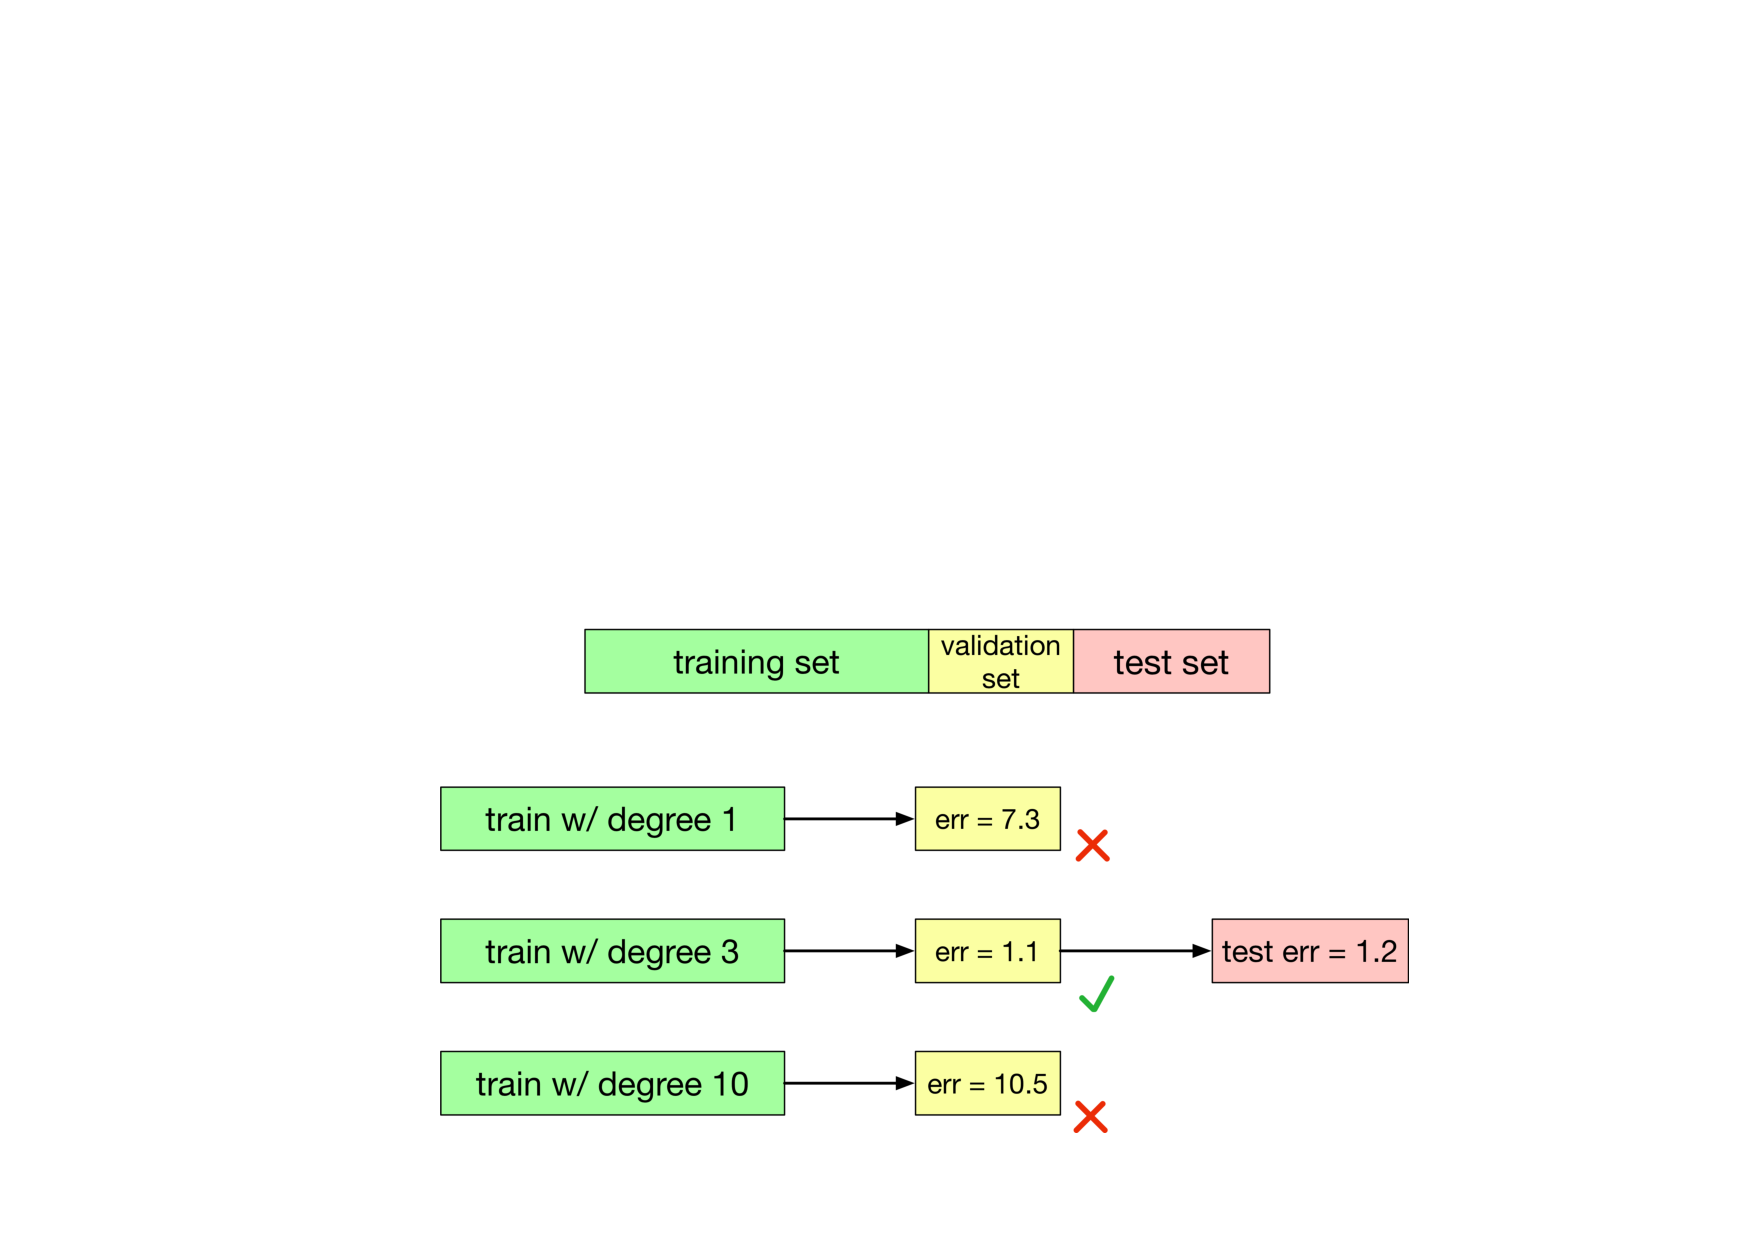
\includegraphics[width=0.9\textwidth]{graphics/validation_set_tuning}
\par\end{center}

\foilhead{Correlation vs. Causation}

\begin{tcolorbox}[colback=red!5!white,colframe=red!75!black,title=Warning] 
Correlation does not always imply causation.
\end{tcolorbox}

\bigskip{}

\bigskip{}

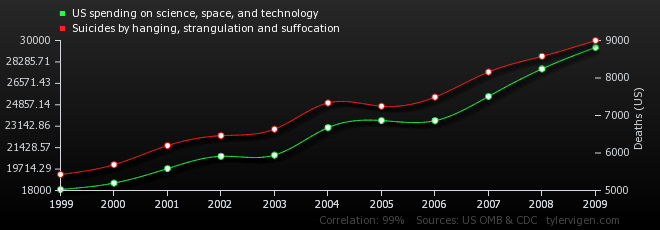
\includegraphics[width=1\textwidth]{graphics/us-spending-on-science-space-and-technology_suicides-by-hanging-strangulation-and-suffocation}

\foilhead{References}
\begin{enumerate}
\item C. M. Bishop, \emph{Pattern Recognition and Machine Learning,} Springer,
2006. (\textcolor{blue}{downloadable})
\item G. James, D. Witten, T. Hastie, R. Tibshirani. \emph{An Introduction
to Statistical Learning with Applications in R.} Springer. 2013. (\textcolor{blue}{downloadable})
\item M. Asch. \emph{Digital Twins: from Model-Based to Data-Driven.} SIAM,
2022. (\textcolor{blue}{extracts})
\end{enumerate}

\end{document}
